\documentclass[]{article}

\usepackage{cite}
\usepackage{amsmath}
\usepackage[letterpaper, margin=1in]{geometry}
\usepackage{graphicx}
\usepackage{mhchem}
\usepackage{upgreek}
\usepackage{braket}

\newcommand\nt{\textup{\scriptsize{0}}}
\newcommand\total{\textup{\scriptsize{total}}}
\newcommand\el{\textup{\scriptsize{el}}}
\newcommand\inel{\textup{\scriptsize{inel}}}
\newcommand\elin{\textup{\scriptsize{el,in}}}
\newcommand\inelin{\textup{\scriptsize{inel,in}}}
\newcommand\out{\textup{\scriptsize{out}}}
\newcommand\PI{\textup{\scriptsize{PI}}}
\newcommand\noscat{\textup{\scriptsize{noscat}}}
\newcommand\sel{\textup{\scriptsize{1el}}}
\newcommand\elpl{\textup{\scriptsize{el,plural}}}
\newcommand\innoinel{\textup{\scriptsize{in,noinel}}}
\newcommand\signal{\textup{\scriptsize{signal}}}
\newcommand\inelpc{\textup{\scriptsize{inel,pc}}}
\newcommand\selpc{\textup{\scriptsize{1el,pc}}}
\newcommand\elplpc{\textup{\scriptsize{el,plural,pc}}}

\newcommand\elb{\textup{\scriptsize{el,\textit b}}}
\newcommand\inelb{\textup{\scriptsize{inel,\textit b}}}
\newcommand\elinb{\textup{\scriptsize{el,in,\textit b}}}
\newcommand\inelinb{\textup{\scriptsize{inel,in,\textit b}}}
\newcommand\outb{\textup{\scriptsize{out,\textit b}}}
\newcommand\PIb{\textup{\scriptsize{PI,\textit b}}}
\newcommand\noscatb{\textup{\scriptsize{noscat,\textit b}}}
\newcommand\selb{\textup{\scriptsize{1el,\textit b}}}
\newcommand\elplb{\textup{\scriptsize{el,plural,\textit b}}}
\newcommand\innoinelb{\textup{\scriptsize{in,noinel,\textit b}}}
\newcommand\inelpcb{\textup{\scriptsize{inel,pc,\textit b}}}
\newcommand\elplpcb{\textup{\scriptsize{el,plural,pc,\textit b}}}
\newcommand\innoinelpcb{\textup{\scriptsize{in,noinel,pc,\textit b}}}
\newcommand\selpcb{\textup{\scriptsize{1el,pc,\textit b}}}
\newcommand\inb{\textup{\scriptsize{in,\textit b}}}
\newcommand\inpcb{\textup{\scriptsize{in,pc,\textit b}}}

\newcommand\elf{\textup{\scriptsize{el,\textit f}}}
\newcommand\inelf{\textup{\scriptsize{inel,\textit f}}}
\newcommand\elinf{\textup{\scriptsize{el,in,\textit f}}}
\newcommand\inelinf{\textup{\scriptsize{inel,in,\textit f}}}
\newcommand\outf{\textup{\scriptsize{out,\textit f}}}
\newcommand\PIf{\textup{\scriptsize{PI,\textit f}}}
\newcommand\noscatf{\textup{\scriptsize{noscat,\textit f}}}
\newcommand\self{\textup{\scriptsize{1el,\textit f}}}
\newcommand\selff{\textup{\scriptsize{1el/f,\textit f}}}
\newcommand\elplf{\textup{\scriptsize{el,plural,\textit f}}}
\newcommand\innoinelf{\textup{\scriptsize{in,noinel,\textit f}}}
\newcommand\inelpcf{\textup{\scriptsize{inel,pc,\textit f}}}
\newcommand\elplpcf{\textup{\scriptsize{el,plural,pc,\textit f}}}
\newcommand\innoinelpcf{\textup{\scriptsize{in,noinel,pc,\textit f}}}
\newcommand\selpcf{\textup{\scriptsize{1el,pc,\textit f}}}
\newcommand\selfpcf{\textup{\scriptsize{1el/f,pc,\textit f}}}
\newcommand\inff{\textup{\scriptsize{in,\textit f}}}
\newcommand\inpcf{\textup{\scriptsize{in,pc,\textit f}}}

\newcommand\micron{$\upmu$m}


\title{X-ray microscopy for thick biological specimens}

\begin{document}

\maketitle

\begin{abstract}

\end{abstract}

\section{Introduction}

\section{X-ray interactions}

\paragraph{} The probability for a photon-matter interaction event (either scattering or photoionization) to occur over a fractional penetration depth \textit{dt} can be expressed as
\begin{equation}
P = \sigma_{i} \rho dt
\end{equation}
where $\sigma_{i}$ is the scattering cross section for interaction event \textit{i}, and $\rho$ is the sample density. This report is concerned with interaction events subdivided into elastic scattering, inelastic scattering, and photoionization, with their cross sections respectively represented by $\sigma_{\el}$, $\sigma_{\inel}$, and $\sigma_{\PI}$. To tidy up the narrative, we also denote
\begin{align}
K_{\el} &= \sigma_{\el}\rho \\
K_{\inel} &= \sigma_{\inel}\rho \\
K_{\elin} &= \sigma_{\el}(1-\eta)\rho \\
K_{\inelin} &= \sigma_{\inel}(1-\eta)\rho
\label{eq:inelin} \\
K_{\out} &= \sigma_{\el}\eta\rho + \sigma_{\inel}\eta\rho \\
K_{\PI} &= \sigma_{\PI}\rho
\end{align}
where $\eta$ is the probability that a photon is backscattered (and thus becomes undetectable) in an elastic scattering event. All cross section data are retrieved from \textit{Xraylib}, a multi-platform database for X-ray-matter interactions \cite{Schoonjans:2011km}. The spatial distribution of scattered X-ray is given by the atomic form factor
\begin{equation}
F(\theta, \phi) = -\tilde{f}r_e\sqrt{1-\textup{sin}^2\theta \textup{cos}^2\phi}.
\end{equation}
For soft x-ray the angular dependence of scattering factor $\tilde{f}$ is negligible \cite{Lonsdale:1962gz}; moreover, since the square root factor is symmetric in space, $\eta$ can be safely evaluated as 0.5 for elastic scattering. Assuming that inelastic scatterings are isotropic, the same evaluation can be applied to $\eta$ in Equation \ref{eq:inelin}. A series of differential equations of x-ray intensity in various categories as a function of penetration depth $t$ can thereby be written \cite{Jacobsen:1998vj}:

\begin{itemize}

\item The intensity component due to photons that do not undergo any interaction with the sample, $I_{\noscat}$, is given according to
\begin{equation}
dI_{\noscat} = -I_{\noscat}(K_{\inel}+K_{\el}+K_{\PI}) dt.
\end{equation}
with initial condition $I_{\noscat}$(0) = $I_{\nt}$.

\item The component of photons that undergo only one elastic scattering event and remain in the detectable angular range, $I_{\sel}$, is given according to
\begin{equation}
dI_{\sel} = I_{\noscat}K_{\elin} dt - I_{\sel}(K_{\inel}+K_{\el}+K_{\PI}) dt
\end{equation}
with $I_{\sel}$(0) = 0.

\item For the component corresponding to photons undergoing multiple elastic scattering events yet still detectable, $I_{\elpl}$, the differential equation is
\begin{equation}
dI_{\elpl} = I_{\sel}K_{\elin} dt - I_{\elpl}(K_{\out}+K_{\inelin}+K_{\PI}) dt
\end{equation}
with $I_{\elpl}$(0) = 0.

\item For photons that are scattered out of the detectable angular range (backscattered), either elastically or inelastically, the corresponding intensity contribution $I_{\out}$ satisfies
\begin{equation}
dI_{\out} = (I_{\nt} - I_{\out} - I_{\PI})K_{\out} dt
\end{equation}
with $I_{\out}$(0) = 0.

\item For photons that are absorbed via photoionization, the component $I_{\PI}$ satisfies
\begin{equation}
dI_{\PI} = (I_{\nt} - I_{\out} - I_{\PI})K_{\PI} dt
\end{equation}
with $I_{\PI}$(0) = 0.

\item The portion of detectable photons that do not undergo inelastic scattering, i.e., the summation of $I_{\noscat}$, $I_{\sel}$, and $I_{\elpl}$, is denoted as $I_{\innoinel}$ and given by
\begin{equation}
dI_{\innoinel} = -I_{\innoinel}(K_{\inelin}+K_{\out}+K_{\PI})
\end{equation}

\item Lastly, $I_{\inel}$, the contribution of photons that undergo at least one inelastic scattering yet are still within the detectable angular range, is given in
\begin{equation}
dI_{\inel} = I_{\innoinel}K_{\inel} dt - I_{\inel}(K_{\out}+K_{\PI}) dt
\end{equation}
with $I_{\inel}$(0) = 0.

\end{itemize}

\begin{figure}[!b]
\begin{center}
\includegraphics[scale=.6]{epsilon.eps}
\caption{Illustration of the geometric model used for calculating $\epsilon$ for a sample with thickness $t$ and an imaging system with pixel size \textit{$\Delta$}, dimension of field of view $N$, and working distance $a$.}
\label{fig:model}
\end{center}
\end{figure}

\paragraph{} Solutions to these differential equations yield
\begin{align}
I_{\noscat} &= I_{\nt}e^{-(K_{\inel}+K_{\el}+K_{\PI})t}
\label{x1} \\
\begin{split}
\label{x2}
I_{\sel} &= I_{\nt}K_{\elin}e^{-(K_{\inel}+K_{\el}+K_{\PI})t} \\
	&= K_{\elin}tI_{\noscat}
\end{split} \\
I_{\elpl} &= I_{\nt} \Big[ e^{-(K_{\out}+K_{\inelin}+K_{\PI})t} - (1+K_{\elin}t)e^{-(K_{\inel}+K_{\el}+K_{\PI})t} \Big]
\label{x3} \\
I_{\out} &= \frac{I_{\nt}K_{\out}}{K_{\out}+K_{\PI}} \Big[1 - e^{-(K_{\out}+K_{\PI})t}\Big]
\label{x4} \\
I_{\PI} &= \frac{I_{\nt}K_{\PI}}{K_{\out}+K_{\PI}} \Big[1 - e^{-(K_{\out}+K_{\PI})t}\Big]
\label{x5} \\
I_{\innoinel} &= I_{\nt}e^{-(K_{\inelin}+K_{\out}+K_{\PI})t}
\label{x6} \\
I_{\inel} &= I_{\nt}\Big[e^{-(K_{\out}+K_{\PI})t} - e^{-(K_{\inelin}+K_{\out}+K_{\PI})t)}\Big].
\label{x7}
\end{align}
It can be demonstrated that
\begin{equation}
I_{\noscat} + I_{\sel} + I_{\elpl} + I_{\out} + I_{\PI} + I_{\inel} = I_{\nt}.
\end{equation}

\paragraph{} In the specific case of X-ray phase contrast imaging, more useful categories can be lined out based on the above results. Firstly, the photons that constitute the image signals are, in addition to non-scattered photons, those having undergone single elastic scattering with the scattering angle within in the range defined by the numerical aperture (NA). Here we consider an NA required for 1 $\upmu$m resolution according to the Abbe criterion. The intensity of this portion of photons, $I_{\selpc}$, is related to $I_{\sel}$ by
\begin{equation}
I_{\selpc} = I_{\sel} \frac{\int_{0}^{s(2\theta=\it{NA})}I(s)ds}{\int_{\textup{forward}}I(s)ds}
\label{eq:frac1}
\end{equation}
where $s$ is the momentum transfer of scattering, $s$ = $4\pi\sin(\theta)/\lambda$, 2$\theta$ is the scattering angle, and $I(s)$ is the scattering intensity as a function of $s$. The upper integral is over the $s$ range stipulated by NA, while the lower is over the regime of forward scattering. We performed data fitting on the small angle X-ray scattering (SAXS) data of 79 different protein samples retrieved from Small Angle Scattering Biological Data Bank (SASBDB) \cite{Valentini28102014} to parameterize $I(s)$, where the normalized Guinier's law
\begin{equation}
I(s) = \exp(-\frac{1}{3}R_g^2s^2)
\label{eq:guinier}
\end{equation}
is applied to the portion with $s$ $<$ 1.3/$R_g$, while a polynomial approximation from the negative fourth to the zeroth order of $s$ is used to model the high-angle portion. $s$ = 3.0 is set as a cut-off point beyond which $I(s)$ is evaluated as 0 to take out the unphysical increasing part of the polynomial. This yields the integrable expression for $I(s)$ which can be plugged into Equation (\ref{eq:frac1}):

\begin{equation}
I(s) = 
\begin{cases} 
      \exp(-1.396s^2) & 0 \leq s < 0.311 \\
      0.0168s^{-4} - 0.1514s^{-3} + 0.4397s^{-2} - 0.2441s{-1} + 0.0399 & 0.311 \leq x < 3.0 \\
      0 & x \geq 3.0. \\
   \end{cases}
\label{eq:fit}
\end{equation}
Taking the $\pm90^{\circ}$-out-of-phase interfering amplitudes of $I_{\noscat}$ and $I_{\selpc}$ yields the signal intensity:
\begin{equation}
I_{\signal} = \sqrt{I_{\noscat}I_{\selpc}}.
\end{equation}

\begin{figure}[!t]
\begin{center}
\includegraphics[scale=.6]{unimatrix_fig.pdf}
\caption{Normalized intensity profiles for X-ray in protein as a function of thickness at incident energy of (a) 5 keV, (b) 10 keV, (c) 20 keV, and (d) 40 keV.}
\label{fig:protein_x_cate}
\end{center}
\end{figure}

Furthermore, if one assumes that inelastic and plural elastic scattering events completely randomize the direction of photons, then the intensity of photons of such kinds that are collected by the objective and thus contribute to the background of phase contrast imaging, $I_{\inelpc}$ and $I_{\elplpc}$, can be calculated from $I_{\inel}$ and $I_{\elpl}$ purely on geometric basis:
\begin{align}
I_{\inelpc} &= I_{\inel}\frac{\pi (\it{NA})^2}{2\pi} \\
I_{\elplpc} &= I_{\elpl}\frac{\pi (\it{NA})^2}{2\pi}.
\end{align}
The above equations are based on the assumption that the working distance $a$ is much larger than the dimension of the field of view $N\Delta$ (Figure \ref{fig:model}) so the offset of the scattering center to the axis is negligible. 

\paragraph{} To simulate biological imaging, the sample is assumed to be a homogeneous block of protein with a composition of \ce{H_{48.6}C_{32.9}N_{8.9}O_{8.9}S_{0.6}} and a dry density of 1.35 \ce{g/cm^2}. This is the effective protein formula proposed by London through averaging over all 20 amino acids \cite{London:1989hh}. Figure \ref{fig:protein_x_cate} shows the intensity profiles relative to sample thickness at varying energies. 

\section{Electron interactions}

\paragraph{} It should be noted that electrons differ from X-ray in that they are never simply absorbed, which negates the presence of the absorption category. Moreover, one may make a general assumption on the fraction of detectable and image-forming electrons, based on a representative cutoff frequency of the aperture of $s_0$ = 4.12 $\mathrm{nm}^{-1}$ proposed by Langmore and Smith \cite{Langmore:1992kk}

\begin{equation}
\eta \approx 1 - \frac{s_0}{10}.
\end{equation}
Equations \ref{x1} to \ref{x7} are then rewritten as
\begin{align}
I_{\noscat} &= I_{\nt}e^{-(K_{\inel}+K_{\el})}
\label{e1} \\
\begin{split}
\label{e2}
I_{\sel} &= I_{\nt}K_{\elin}e^{-(K_{\inel}+K_{\el})t} 
	\\ &= K_{\elin}tI_{\noscat} 
\end{split} \\
I_{\elpl} &= I_{\nt} \Big[ e^{-(K_{\out}+K_{\inelin})t} - (1+K_{\elin}t)e^{-(K_{\inel}+K_{\el})t} \Big]
\label{e3} \\
I_{\out} &= I_{\nt} \Big(1 - e^{-K_{\out}t}\Big)
\label{e4} \\
I_{\innoinel} &= I_{\nt}e^{-(K_{\inelin}+K_{\out})t}
\label{e6} \\
I_{\inel} &= I_{\nt}\Big[e^{-K_{\out}t} - e^{-(K_{\inelin}+K_{\out})t)}\Big].
\label{e7}
\end{align}

\begin{figure}[b!]
\begin{center}
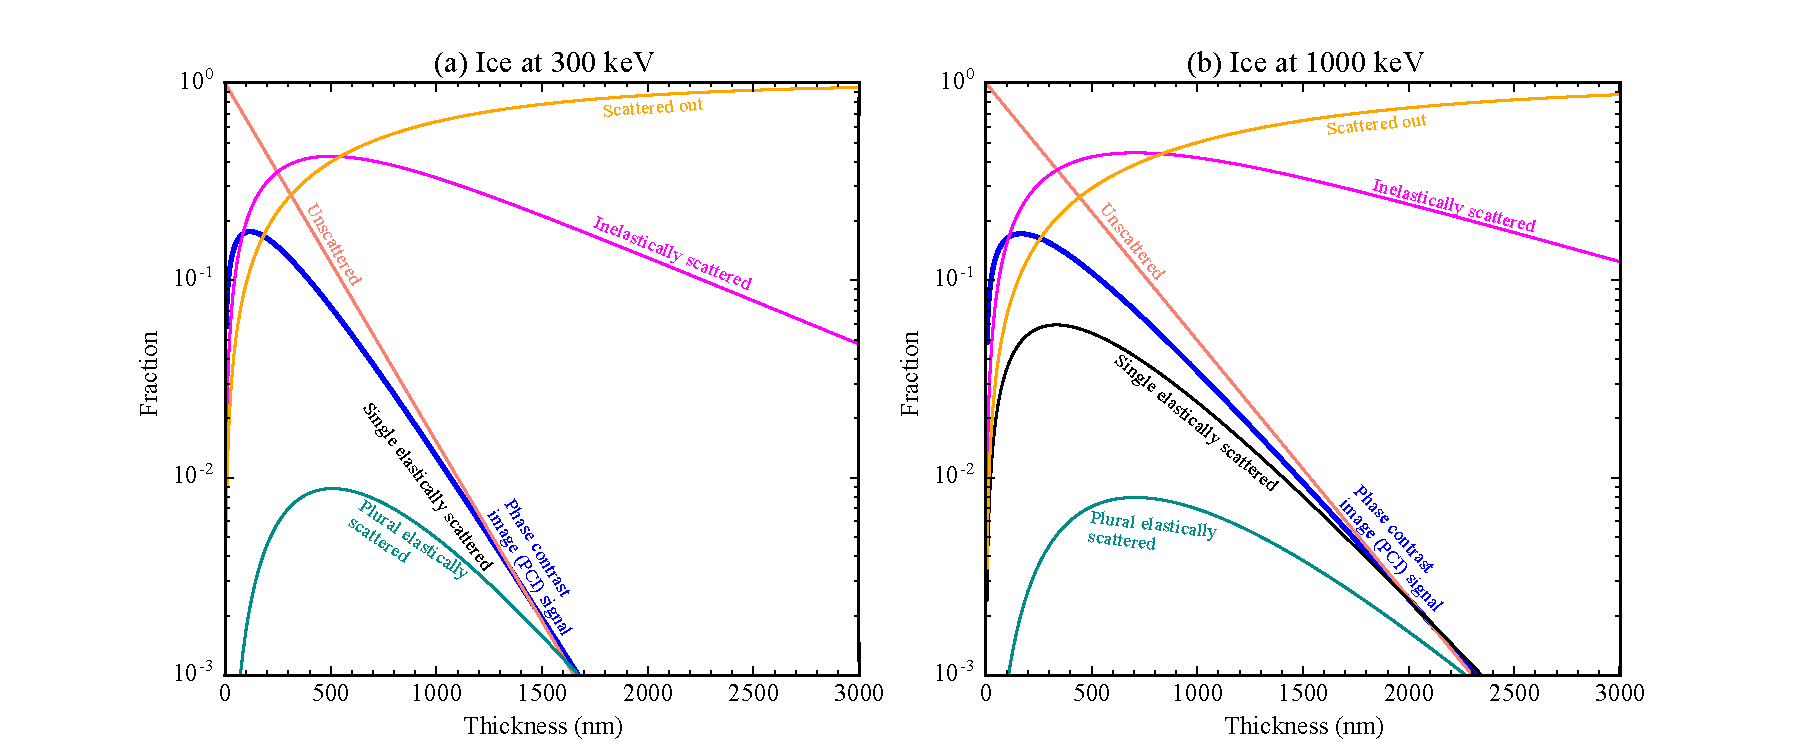
\includegraphics[scale=0.6]{unimatrix_fig_e.pdf}
\caption{Normalized intensity profiles for electrons in vitreous ice as a function of thickness at incident energy of 300 keV. Reproduced from Jacobsen et al. (1998) with permission.}
\label{fig:ice_e_cate}
\end{center}
\end{figure}

\paragraph{} Based on the model, Jacobsen et al. \cite{Jacobsen:1998vj} have considered the case where a heavily hydrated specimen is embedded in vitreous ice. The ice layer is assumed to be so thick that one may use the scattering cross sections for \ce{H2O} throughout the entire sample. A reproduction of their work for electrons with energy 300 keV and 1000 keV is shown in Figure \ref{fig:ice_e_cate}. 

\section{Contrasting X-ray and electron microscopy on radiation dose}

\paragraph{} The categorization of X-ray and electron beam intensities would immediately answer our questions on the image contrast and the radiation dose to the specimen. For both probe types we consider a finer model proposed by Jacobsen et al. \cite{Jacobsen:1998vj} where a protein layer with thickness $t_f$ is embedded in ice with thickness $t_b$, and rewrite the intensity equations to separately account for the background (from ice) and signal (from protein) intensity categories. Here we only present the modified model for X-ray as follow:
\begin{align}
I_{\noscatb} &= I_{\nt}e^{-(K_{\inelb}+K_{\elb}+K_{\PIb})t}
\label{xb1} \\
\begin{split}
\label{xb2}
I_{\selb} &= I_{\nt}K_{\elinb}e^{-(K_{\inelb}+K_{\elb}+K_{\PIb})t} \\ 
	&= K_{\elinb}t I_{\noscatb}
\end{split} \\
I_{\innoinelb} &= I_{\nt}e^{-(K_{\inelinb}+K_{\outb}+K_{\PIb})t}
\label{xb3} \\
I_{\elplb} &= I_{\innoinelb} - I_{\noscatb} - I_{\selb}
\label{xb4} \\
I_{\inb} &= I_{\nt}e^{-(K_{\outb}+K_{\PIb})t} 
\label{xb5} \\
I_{\inelb} &= I_{\inb} - I_{\innoinelb}
\label{xb7} \\
I_{\inelpcb} &= I_{\inelb} \frac{\pi(NA)^2}{2\pi} \\
I_{\elplpcb} &= I_{\elplb} \frac{\pi(NA)^2}{2\pi}
\end{align} % --------------------
and
\begin{align}
I_{\noscatf} &= I_{\nt}e^{-(K_{\inelb}+K_{\elb}+K_{\PIb})t_b}e^{-(K_{\inelf}+K_{\elf}+K_{\PIf})t_f}
\label{xf1} \\
I_{\self} &= (K_{\elinb}t_b + K_{\elinf}t_f) I_{\noscatf}
\label{xf2} \\
I_{\selff} &= K_{\elinf}t_f I_{\noscatf}
\label{xf2.5} \\
I_{\innoinelf} &= I_{\nt} e^{-(K_{\outb}+K_{\inelinb}+K_{\PIb})t_b} e^{-(K_{\outf}+K_{\inelinf}+K_{\PIf})t_f}
\label{xf3} \\
I_{\elplf} &= I_{\innoinelf} - I_{\noscatf} - I_{\self}
\label{xf4} \\
I_{\inff} &= I_{\nt}e^{-(K_{\outb}+K_{\PIb})t}e^{-(K_{\outf}+K_{\PIf})t}
\label{xb5} \\
I_{\inel} &= I_{\inff} - I_{\innoinelf}.
\label{xf7} \\
I_{\inelpcf} &= I_{\inelf} \frac{\pi(NA)^2}{2\pi} \\
I_{\elplpcf} &= I_{\elplf} \frac{\pi(NA)^2}{2\pi} 
\end{align} % --------------------
Furthermore, the intensities of X-ray after passing matrix-only ($I_{\innoinelpcb}$ and $I_{\inpcb}$; the former excluding inelastically scattered photons while the latter counting in this category) and feature-containing ($I_{\innoinelpcb}$ and $I_{\inpcb}$) columns in the specimen, are written as 
\begin{align}
I_{\innoinelpcb} &= I_{\noscatb} + I_{\selb} + I_{\elplpcb} \\
I_{\inpcb} &= I_{\noscatb} + I_{\selb} + I_{\elplpcb} + I_{\inelpcb}
\end{align}
and
\begin{align}
I_{\innoinelpcf} &= I_{\noscatf} + I_{\selpcf} + I_{\elplpcf} \\
I_{\inpcf} &= I_{\noscatf} + I_{\selpcf} + I_{\elplpcf} + I_{\inelpcf}
\end{align}
where $I_{\selpcf}$ is obtained using the same approach as in Equation \ref{eq:frac1} and \ref{eq:fit}. For the small-molecule matrix, we take the low-$R_g$ limit of Guinier's law (Equation \ref{eq:guinier}) to find out that the curve would theoretically be very flat and smooth, which has an overall agreement with experimental results for water \cite{Hedlund:2009ix}. It is thus reasonable to assume a constant intensity distribution with regard to the reciprocal space variable $s$, thus 
\begin{equation}
I_{\selpcb} = \frac{NA}{2\sin(\pi/4)}I_{\selb}
\end{equation}

\paragraph{} From the matrix-feature dichotomy, the signal and noise of the resultant image can be straightforwardly written as 
\begin{align}
S &= N|I_f-I_b| \\
N &= \sqrt{N}\sqrt{I_f+I_b}
\end{align}
where $N$ is the number of probe particles per pixel. Consequently, the signal-to-noise ratio (SNR) is given by \cite{Sun:2015fr}
\begin{equation}
\begin{aligned}
\textit{SNR} &= \sqrt{N}\frac{I_f-I_b}{\sqrt{I_f+I_b}} \\ &= \sqrt{N}\Theta
\end{aligned}
\end{equation}
where $\Theta$ is the image contrast. For X-ray phase contrast imaging, this factor is expressed as
\begin{equation}
\Theta_\mathrm{x} = \frac{|I_{\innoinelpcf}-I_{\innoinelpcb}|+2\sqrt{I_{\noscatf}I_{\selfpcf}}}{\sqrt{I_{\inpcf}+I_{\inpcb}}}
\end{equation}
where $I_{\selfpcf}$ is the in-NA portion of single elastically scattered photons that are scattered by and only by protein features. For the electron counterpart, we consider both cases where an energy filter, assumed to be capable of blocking out all inelastically scattered electrons, is used or not:
\begin{align}
\Theta_{\mathrm{e,unfiltered}} &= \frac{|I_{\innoinelf}-I_{\innoinelb}|+2\sqrt{I_{\noscatf}I_{\selff}}}{\sqrt{I_{\inff}+I_{\inb}}} \\
\Theta_{\mathrm{e,filtered}} &= \frac{|I_{\innoinelf}-I_{\innoinelb}|+2\sqrt{I_{\noscatf}I_{\selff}}}{\sqrt{I_{\innoinelf}+I_{\innoinelb}}}
\end{align}
where $I_{\inff} = I_{\innoinelf} + I_{\inelf}$ and $I_{\inb} = I_{\innoinelb} + I_{\inelb}$. According to the Rose criterion which states that a SNR of of at least 5 is required for precise identification of image features, $N$ should be
\begin{equation}
N = \frac{25}{\Theta^2}.
\end{equation}
It is further notice that, since for X-ray the probability of absorption almost always predominates over all interaction events, we can neglect the energy deposition due to inelastic scattering, and write the specimen radiation dose in Gray (J/kg) for X-ray as 
\begin{equation}
D_\mathrm{x} = \frac{NE}{\Delta^2 \Lambda_{\PI,f} \rho}
\end{equation}
where $E$ is the incident photon energy, $\Delta$ is the pixel size (which defines the resolution in scanning X-ray microscopy), and $\Lambda_{\PI,f} = 1/K_{\PI,f}$ is the mean free path with regards to photonionizational absorption in the feature material. In the case of electron, the radiation dose is contributed by inelastic scattering only:
\begin{equation}
D_\mathrm{e} = \frac{N\Braket{E}}{\Delta^2 \Lambda_{\inel,f} \rho}
\end{equation}
where $\Lambda_{\inel,f}$ is analogous to its absorption counterpart, and $\Braket{E}$ is the expectation of energy deposition in an inelastic scattering event, evaluated from the electron energy-loss spectra (EELS) for ice as 39.3 eV and for protein as 37.5 eV \cite{Isaacson:1975wr}. In this work, we visualize the variation of radiation dose with the total thickness for a 10 nm embedded protein layer, imaged with using soft (500 eV) and hard (10 keV) X-ray and 300 keV electrons with and without energy filter (Figure \ref{fig:dose}). 

\begin{figure}[t!]
\begin{center}
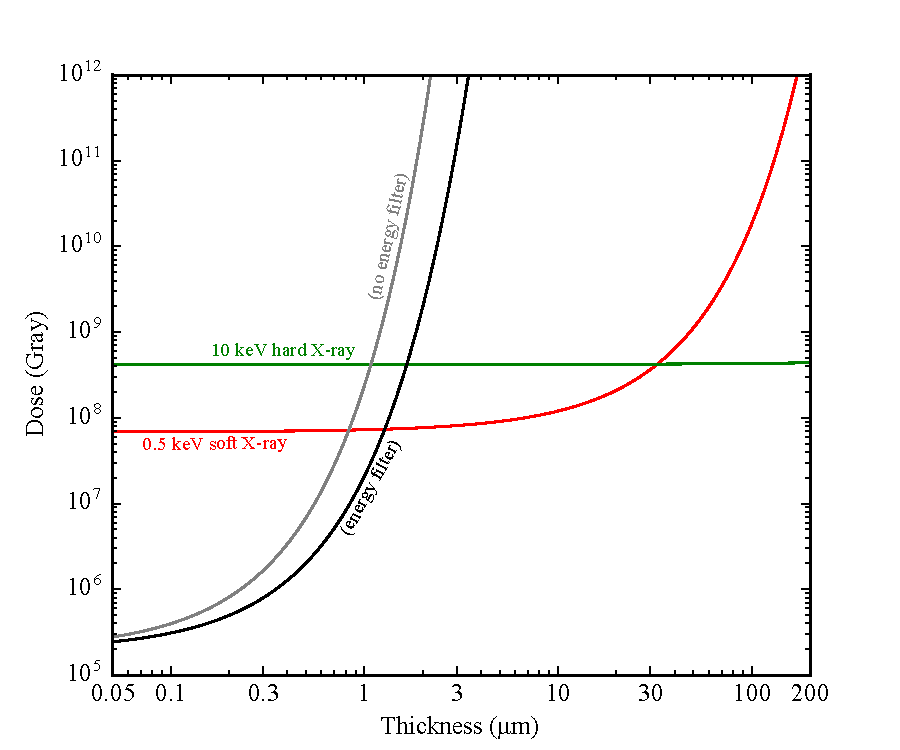
\includegraphics[scale=0.7]{dose.pdf}
\caption{Radiation dose at varying specimen thickness for 0.5 keV soft X-ray and 10 keV hard X-ray, in comparison with 300 keV electrons, with and without energy filter.}
\label{fig:dose}
\end{center}
\end{figure}

\paragraph{} The paradigm scenario illustrated here indicates a general tendency that soft X-ray produces lower radiation dose than electrons. This advantage, however, is counterbalanced by the high spatial resolution that electron microscopy can provide, and diminishes when the specimen thickness is on or beyond the order of 10 \micron. Increasing the energy of X-ray would effectively reduce the sensitivity of radiation dose to ice thickness. Electron microscopy proves superiority for specimen thickness within the sub-100-nm regime; however, for thickness beyond 300 nm, the ratio of multiple scattering or inelastic scattering over single elastic scattering events begins to take off, which, on the other hand, remains steady for X-ray. Thus, when resolution is not a strict requirement, X-ray is a less intrusive technique for imaging biological specimens. 



\section{Acknowledgement}
\paragraph{} The authors would like to thank the developers and contributors of \textit{Xraylib} and SASBDB for supplying a substantial portion of the data used in this work. 

\bibliography{mybib}{}
\bibliographystyle{ieeetr}

\end{document}